\chapter{Quadratic Functions}
\label{ch:quadfunc}

\chapquote{Nature creates curved lines while humans create straight lines.}{Hideki Yukawa\\Japanese theoretical physicist}

In the last few chapters, we have studied quadratic equations, the methods for solving them, and the various algebraic rules for manipulating the kinds of answers we get (square roots). We turn now to quadratic relationships and situations that can be represented using quadratic functions. We'll look more closely at the equations and graphs of quadratic functions, and look closely at one of the classic applications from physics.

% % % % % % % % % % % % % % % % % % % % % % % % % % % % % % % % % % % % % % % % 
\section{Quadratic Relationships}
\label{sec:quadrelationships}

\begin{boxedexplore}[Extended Exploration: Staking a Claim]
LINK
\end{boxedexplore}

\begin{boxedexplore}[Startup Exploration: Compost Heap]
Uncle Fran\c{c}ois wants to make a compost heap in the corner of his vegetable garden. He plans to enclose a rectangular area using the two existing walls of the garden, plus 8 yards of leftover fencing.

\begin{center}
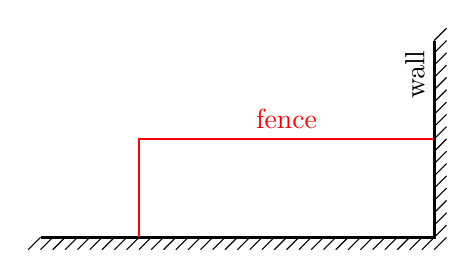
\begin{tikzpicture}[scale=0.625]
	\draw[very thick] (0,0) -- (8,0) -- (8,4);
	\draw(8,4) node[rotate = 90, above left]{wall}; 
	\foreach \x in {0, 0.25,...,8.25} \draw (\x,0) -- (\x-0.25, -0.25);
	\foreach \y in {0, 0.25,...,4} \draw (8,\y) -- (8.25, \y+0.25);
	\draw[red, thick] (2,0) -- (2,2) -- node[above]{fence} (8,2);
\end{tikzpicture}
\end{center}

If he wants to enclose the largest possible area, how should he arrange the fence? What is the maximum area he can enclose?
\end{boxedexplore}

Thoughts:

This startup is similar to staking a claim, but I hope different enough. I couldn't come up with a new quadratic scenario that so clearly demonstrated all the features of quadratics (all in the first quadrant) AND had such a natural way to write the equation.

The plan will be to do the staking a claim treatment with this problem and hit the highlights about symmetry, the vertex, and all that.


% % % % % % % % % % % % % % % % % % % % % % % % % % % % % % % % % % % % % % % % 
%\section{Introduction to Quadratic Functions}
%\label{sec:quadintro}
%
%
%
%Vocabulary
%
%Parabola The U-shaped graph of a quadratic function. There is the geometric definition:
%the set of all points the same distance from a fixed point called a focus and a line
%called a directrix.
%
%Vocabulary
%
%Axis of Symmetry The line that passes through the vertex and divides the parabola into two
%symmetric parts.
%
%Vocabulary
%
%Vertex The lowest or highest point on a parabola
%
%Vocabulary
%
%Standard Form of a Quadratic Function A quadratic function in the form y = ax2 + bx + c,
%where a \$ eq\$ 0
%
%
%Vocabulary
%
%Vertex Form A quadratic function in the form y - k = a(x - h)2 or y = a(x - h)2 + k ,
%where (h, k) is the vertex.
%
%Vocabulary
%
%Factored Form A quadratic function in the form y = (ax + b) (cx + d), where a and c
%$\neq$ 0. Related to intercept form which is y = a(x-r1)(x-r2) where r1 and r2 are the
%roots (x-intercepts) of the related quadratic equation.
%
%Vocabulary
%
%Second Difference When a table of values shows domain values that are sequential integers,
%the second difference is the difference of the difference of the independent variable's
%values. The second difference of a quadratic function is constant.
%
%Vocabulary
%
%Quadratic Function A nonlinear function that can be written in the standard form y = ax2 +
%bx + c, where a \$ eq\$ 0
%
%Vocabulary
%
%Maximum Value For y = ax2 + bx + c where a <0, the y-coordinate of the vertex is the
%maximum value of the function.
%
%Vocabulary
%
%Minimum Value For y = ax2 + bx + c where a >0, the y-coordinate of the vertex is the
%maximum value of the function.
%
%Vocabulary
%
%Fixed Perimeter A set perimeter that can't change due to given constraints.
%
%Staking a Claim --> Introduction
%
%Today you begin your study of the last family of functions for Algebra 1, the Quadratic
%Function. By the end of the lesson, you are going to know the characteristics of
%quadratics as they appear in tables, graphs and equations. You are going to use one of the
%classics examples of quadratic relationships to achieve this, the fixed perimeter problem.
%
%Follow-Up From Staking a Claim (Data and Tables)
%
%1. What is the domain of the function represented in the table? * If x = length, (integers
%or real) 0 < x < 20 * In general, quadratics have the domain of all reals
%
%2. What is the range of the function represented in the table? * If y = area, (integers or
%real) 0 < y $\leq$ 100 * In general, quadratics have two ranges Y $\leq$ Maximum
%Y $\geq$ Minimum
%
%3. Should we include length and widths of zero? * Yes, because when I extend the domain to
%include the rational numbers, I need to have those as boundaries.
%
%4. What properties does the table have? * Symmetric --> where does the line of symmetry
%occur? At x = 10 * Increases, hits a maximum area, then decreases --> in general they can
%also decrease, hit a minimum, then increase * The rate at which it increases slows down.
%It is not constant. If it were it would be a line. * In general, if the Independent
%Variable values are sequential, this will be true at some point in the table. You can't
%rely on this ``increases then decreases'' (or the reverse) to determine if a table is
%quadratic. You might not get that part of the table that shows that, so we have to look
%more closely at the pattern
%
%5. What are some of the patterns that you notice? * Increase, hits a maximum value, then
%decreases --> in general, it can also Decrease, hits a minimum value, then increase * Rate
%of change is not constant, but changes in a pattern . The pattern just happens to be
%linear!--> most important part of this!!!! * Second Difference is Constant (and not = to
%zero)--> true for all quadratics and it is the test to determine if a table represents a
%quadratic relationship. This is what creates the familiar curve in the graph. * In
%general, the sign of the second difference will tell if the parabola is going to increase
%then decrease (sad parabola = negative 2nd difference) or if it is going to decrease then
%increase (happy parabola = positive 2nd difference)
%
%6. How do we know that the table is quadratic? * From the pattern activity in the
%beginning of the year, constant second difference
%
%Length Width Area First Diff. Second Diff. 0 20 0 19 17 15 13 11 9 7 5 3 1 -1 -3 -5
%Constantly decreasing rate of change -2 -2 -2 -2 -2 -2 -2 Constant and negative second
%difference.
%
%The table must be sequential to show this. The x's can count by 1, 2, 3, as long as it is
%consistent. 1 19 19
%
%
%2 18 36
%
%
%3 17 51
%
%
%4 16 64
%
%
%5 15 75
%
%
%6 14 84
%
%
%7 13 91
%
%
%8 12 96
%
%
%9 11 99
%
%
%10 10 100
%
%
%11 9 99
%
%
%12 8 96
%
%
%13 7 91
%
%
%Etc.
%
%
%
%
%
%Follow-Up from Staking a Claim (Graphs)
%
%1. What is the domain and range for the graph? --> See above
%
%2. Describe the shape of the graph. * It is a function (passes the vertical line test) *
%Parabola --> U-shaped
%
%3. What are some special features of the graph? * It has a maximum value --> parabola with
%a maximum (aka opens down or sad parabola) * This maximum/minimum is called the Vertex *
%In general, it can also have a minimum value --> parabola with a minimum (aka opens up or
%happy parabola) * The graph is not made up of straight line segments. It is a curve that
%is less steep the closer you get to the vertex. The steepness increases as you move away
%from the vertex. --> true for all parabolas * Has a line of symmetry and the vertex occurs
%at the axis of symmetry --> true for all * Has two x-intercepts that are equidistant from
%the line of symmetry --> true for all that have 2 x-intercepts. In general you can have 0,
%1, or 2 x-intercepts. If there is only one, the vertex is the x-intercept because every
%other time, you get two x's for a single y-value. If you have no x-intercepts, the graph
%starts above or below the x-axis. * There are two y-values for all x-values except for the
%vertex. \ldots{} every point has a buddy on the other side of the line of symmetry except
%for the vertex.
%
%4. What occurs at the axis of symmetry? --> the vertex 5. Can you see these features in
%the table? Yes. There is a line of symmetry, two y's for each x and the rate of change
%dictated the shape of the function
%
%
%
%
%Follow Up From Staking a Claim (Equations)
%
%1. What is one of the equations that will represent this data? And how did you come up
%with it? * Y = x(20-x) * X = length, 20-x = width., multiply length and width to get area
%* This is called the factored form. This shows the relationship as a product. You can only
%have this form if the graph has x-intercepts! --> hint for the future, if we can write a
%quadratic in this form, we can very easily find the x-intercepts * Notice that for fixed
%perimeter problems there is a general formula for the area. . 2. How can I turn this into
%a different equation? * Distribute the x * Y = 20x - x2 or Y = -x2 + 20x * This is called
%the standard form. This is the only form (that we are going to study) that you can use for
%all quadratic functions and that the definition of the Quadratic Function is based on this
%specific equation. * The a, b, and c tell you quite a bit about the graph and we will look
%more closely at this next class. * Notice that for fixed perimeter problems, there is a
%general formula of the area or
%
%3. Is there another form? * Of Course! There are several others. One often used in Algebra
%II is called the vertex form. It is the form that uses the vertex right in the equation.
%
%Follow Up From Staking a Claim ( Using Quadratic Functions to solve problems.)
%
%1. What is the greatest possible area? 100 sq yds.
%
%2. What shape is this specifically? A square
%
%3. How can I use the table, graph, equation to answer this? * You are looking for the
%maximum value! The y-value is the maximum area and the corresponding x-values tells you
%the side length of the square. --> In general, you will often have to find the maximum to
%answer a word problem. Sometimes you want y- or x- intercepts too. * Now, the graph
%actually tells me more about fixed perimeters in general. --> see picture below
%
%4. Does opening up the domain to be real numbers (as opposed to integers) change this
%solution?-->No. The graph is the picture of all such rectangles. The data points in
%between the ones that were graphed are those with non-integer side lengths. So, the
%maximum is still the maximum.
%
%5. What shape would I use if I really wanted to maximize area? --> A circle! The perimeter
%is fixed, no matter what. The more sides you add to that polygon, the bigger the area is
%going to be. So a regular hexagon will have a greater area than a square with the same
%perimeter. If you extend this reasoning, then a regular polygon with infinite sides will
%have the biggest area of them all\ldots{} and that is just a circle!
%

\section{Vertex Form}

%%Like linear functions, quadratic functions have more than one equation form. There are three that we will look at in algebra 1: standard form, vertex form, and factored form (or intercept form).
%%
%%The standard form of a quadratic equation is the one we've seen already:
%%\[y=ax^2 + bx + c\] 
%%
%%Vertex form is the one that is most convenient for graphing
%%
%%Factored form is great for identifying the $x$-intercepts (we'll look at this form in detail in the next chapter)
%%
%%\begin{boxeddef}[Vertex Form]
%%A quadratic equation of the form \[y-k = a(x-h)^2 \quad\OR\quad y=a(x-h)^2+k,\] where the point $(h,k)$ is the vertex of the parabola, and $a$ is a factor controlling the ``steepness'' of the parabola.
%%\end{boxeddef}

Build on transformations to discuss vertex form, and graphing in vertex form.

\section{Graphing Quadratics}

Graphing quadratics in standard form, equation for line of symmetry in standard form, finding vertex in standard form (using LOS).

%What We Know So Far\ldots{}
%
%Standard Form: y = ax2 + bx + c where
%
%The Graphs Features: * They are U-shaped curves called parabolas. * Parabolas are
%symmetric * The vertex (max or min) will occur on the line of symmetry * They can open
%up(happy) or open down (sad) * They have a max if they open down and a min if the open up
%* They can have 0, 1, or 2 x-intercepts (aka roots or zeroes of the function) * If there
%is one x-intercept, it is the vertex * If there are two x-intercepts, they are equidistant
%from the axis of symmetry.
%
%Transformations (what changing a, b, and c do to the graph)
%
%The Parent Function: y = x2 1. a * If a is positive, the parabola opens up * If a is
%negative, the parabola opens down * If the parabola is the same width as the parent * If
%the parabola will be narrower than the parent * If the parabola will be wider than the
%parent 2. b shifts left or right 3. c * This coordinates of the y-intercept are (0, c), if
%you plug in zero for x, you get c for y. * If a value was just added to or subtracted from
%the parent ( y = ax2 + c) , it would move the parabola up or down
%
%Graphing Strategy
%
%Every unique parabola can be created with exactly 3 points. That's why you need 3 data
%points to do a quadratic regression on a calculator.
%
%So, the bare minimum to graph, or define, a parabola is 3 points. (Similarly, lines needed
%two points). So instead of making huge tables that have many points, we are going to find
%a few strategic points to plot so that we can sketch a reasonable curve efficiently.
%
% Points we want: (1) the vertex --> the most important point!!!!!!!!! (2) the y-intercept
% (3) the x-intercept(s).
%
%Remember, parabolas are symmetric. Take advantage of that!
%
%How to Graph
%
%1. Stop to look at your equation and think about what your graph is going to look like by
%looking at the values of a, b, and c 2. Find and plot the Axis of Symmetry --> this tells
%us where to find the vertex, and gives us a way to double the number of additional points
%to plot. 3. Find the vertex --> It is on the Axis of Symmetry, so substitute in that
%x-value to find the y-coordinate. It tells you range\ldots{} SUPER IMPORTANT POINT 4. Find
%the x- and y-intercepts --> If you have a standard form equation, the y-intercept is easy.
%It is that ``c'' value. Finding the x-intercept, now that is tricky. We'll see why in soon
%enough 5. Get any additional points as necessary to sketch a reasonable curve. --> If you
%can't find the x-intercepts, or if the graph doesn't have any, and you need to find
%another point, just substitute in some value of x into the function to find the coordinate
%of another point.
%
%Graphing of the form y = ax2 + c
%
%What are some features that all these graphs? 1. They all have the y-axis as the line of
%symmetry. 2. Their vertices will be their y-intercepts.
%
% Before you start to work predict what the graphs will look like * Is it going to open up
% or down? * Will the vertex be a maximum or a minimum? * Will it be wider or narrower than
% the parent? * Is the line of symmetry the y-axis, or is it shifted?
%
%Example 1
%
%Graph: y = 3x2
%
%Solution: * Should open up, have a minimum, be skinny, and an un-shifted line of symmetry
%* Axis of Symmetry: x = 0 * Coordinates of Vertex: y = 3(0)2 = 0 --> (0,0) * X- and
%Y-intercepts? --> it's vertex is the origin, so I've already found these * Find one other
%point\ldots{} let's plug in x = 1 --> y = 3(1)2 = 3, so plot (1,3). * Reflection across
%the axis of symmetry: (-1,3)
%
%
% Example 2 Graph Solution: * Should open down, have a maximum, be wide, and an un-shifted
% line of symmetry * Axis of Symmetry: x = 0 * Coordinates of Vertex: y = - ? (0)2 = 0 -->
% (0,0) * X- and Y-intercepts? --> it's vertex is the origin, so I've already found these *
% Find one other point\ldots{} let's plug in x = 4 --> y = (- ?) (4)2 = -4, so plot (4,-4).
% * Reflection across the axis of symmetry: (-4,-4)
%
%
%Example 3 Graph y = x2 + 5
%
%Solution: * Should open up, w/ minimum, same width as parent, and un-shifted line of
%symmetry * Axis of Symmetry: x = 0 * Coordinates of Vertex: y = (0)2 +5 = 5 --> (0,5) *
%Y-Intercept --> is the vertex * X-intercept --> replace y with zero and solve for x (by
%definition) --> oops, not real! * Find one other point\ldots{} let's plug in x = 1 --> y
%=(1)2 + 5= 6, so plot (1,6). * Reflection across the axis of symmetry: (-1,6)
%
%
%Example 4
%
%Graph y = 2x2 - 8
%
%Solution: * Should open up, w/minimum, skinny * Axis of Symmetry: x = 0 * Coordinates of
%Vertex: y = 2(0)2 -8 = 8 --> (0,8) * Y-Intercept --> is the vertex * X-intercept -->
%replace y w/0 and solve for x --> use your PoEs \& square rooting skills and you get +/- 2.
%(remember, when you choose to square root, you have to put the sign back on).
%
% Locating the Axis of Symmetry from the Standard Form Equation
%
%Now, what if I throw in that ``bx'', or, linear term? That will shift the axis of
%symmetry, but by how much? There is actually a formula based on the numbers in the
%standard form equation that will find the axis of symmetry.
%
%Equation for Axis of Symmetry of Parabola
%
%Given where a $ eq$0 the equation for the axis of symmetry is .
%
%Example 5
%
%Graph: y = 3x2 - 6x + 2
%
%Solution: 1. Open up, w/minimum, skinny, shifted line of symmetry 2. Axis of Symmetry: 3.
%Coordinates of Vertex: (1, -1)
%
%
%4. Y-Intercept is not the vertex this time --> (0,2) 5. X-intercept --> replace y with
%zero and solve for x (by definition) --> Uh, ewe. We can't find them in this equation.
%Every time we use a POE, we are left with something that we can't solve! Noooo! So, before
%we can plot these, we are going to have to learn a way to deal with that type of equation
%\ldots{} next class period! 6. We have to find other points. We have several options,
%depending on how accurate you want your graph to be * We can find the y-intercept's
%reflection and plot it --> (2,2) * We can plug in x = 3 to find an additional point -->
%use x = 3, and find (3,11) and (-1, 11) * We can do both of the above --> will give us the
%best graph
%
%Example 6
%
%Graph: y = x2 - 4x + 4
%
%Solution: 1. Open up, w/minimum, same width as parent, shifted line of symmetry 2. Axis of
%Symmetry: 3. Coordinates of Vertex: (2,0) --> oooo, the x-intercept!
%
%
%4. X-intercept --> we accidentally found that already 5. Y-Intercept is not the vertex
%this time --> (0,4) 6. We have to find other points. We have several options, depending on
%how accurate you want your graph to be * We can find the y-intercept's reflection and plot
%it --> (4,4)\ldots{} preferred * We can plug in x = 1 , 3, anything but 2 or 0 * We can do
%both of the above --> will give us the best graph
%
%Example 7
%
%Graph: Solution: 1. Opens up, w/minimum, wider, shifted line of symmetry 2.Axis of
%Symmetry: 3. Coordinates of Vertex: (-9,-36)
%
%4.Y-Intercept is not the vertex this time --> (0,-9)
%
%5. X-intercept --> nope, can't do that yet.. but I do know that there are 2\ldots{} it
%opens up and the vertex is below the x-axis 6. We have to find other points. We have
%several options, depending on how accurate you want your graph to be * We can find the
%y-intercept's reflection and plot it --> (-18,-9) * We can plug in x = anything but 9, 1'm
%going to pick 3 * We can do both of the above --> will give us the best graph Example 8
%
%Graph: Solution: 1. opens down, w/maximum, same width as parent, shifted line of symmetry
%2. Axis of Symmetry: 3. Coordinates of Vertex: (-2.5, -0.25)
%
%4. Y-Intercept is not the vertex this time --> (0,-6)
%
%5. X-intercept --> nope, can't do that yet.. but I do know that there are 2\ldots{} it
%opens down and the vertex is above the x-axis 6. We have to find other points. We have
%several options, depending on how accurate you want your graph to be * We can find the
%y-intercept's reflection and plot it --> (-5,-6) * We can plug in x = 3 to find an
%additional point --> use x = -2 or -3, and find \ldots{}oh, the x-intercepts!
%



%Standard --> the one we've been working with most
%2. Vertex --> the best for graphing 3. Factored --> the best for finding x-intercepts,
%which we'll look at last in the quadratic unit
%
%Vertex Form of a Quadratic: or where (h,k) are the coordinates of the vertex. Should look
%a little familiar \ldots{} point-slope anyone?
%
%This form is based on translating (shifting) the vertex of y = ax2 from (0, 0) to (h, k).
%* y = ax2 + k moves the vertex up or down k-units * y = a(x-h)2 moves the vertex left or
%right h units * The width and orientation of y = ax2 and should be the same.
%
%How to use the vertex form to graph.
%
%It gives you the coordinates of the vertex and therefore the location of the line of
%symmetry! That's half the work right there.
%
%Example 1
%
%Problem: What does y - 15 = 3 (x - 8)2 tell you about the graph.
%
%Solution: * The Vertex is located at (8, 15) * The line of symmetry is x = 8 * The 3 tells
%me it is thinner than the parent, opens up and has a minimum * The range of the function
%is y ? 15 * It has no x-intercepts
%
%The only thing I don't know, the location of the y-intercept. But, I can calculate that
%easily by substituting in x = 0 and solving for y.
%
%y - 15 = 3(0-8)2 y = 3(64) + 15 = 207
%
%Unpleasant to graph because of the horrible y-scale, but much easier to find the needed
%information for a graph.
%
%Converting from vertex to standard
%
%Not that you really want to but\ldots{}. Super easy. Just simplify! Don't forget Leo
%B./FOIL Example 2
%
%Problem: Convert
%
%Solution:
%
%
%
%
%Converting from standard to vertex\ldots{}.
%
%Something you really want to be able to do\ldots{} but can't yet. You need to learn a
%process called ``completing the square.'' Before I can teach you that, you have to learn
%about these things called polynomials. Then you have to learn how to factor a polynomial.
%Then you have to learn about these things called perfect square trinomials\ldots{} then
%you can learn how to complete the square. It is one of the last lessons of the year.
%
%

%\section{Solving Quadratics}
%
%Check for completion here...

%
%Vocabulary
%
%Standard Form Quadratic Equation An equation of the form 0 = ax2 + bx + c, where a $ eq$
%0. It has a corresponding function y = ax2 + bx + c. Solving this equation will locate the
%x-intercepts of the corresponding function. Standard form quadratic equations must = 0!
%
%Vocabulary
%
%Quadratic Formula A formula that uses the coefficients of the terms of a standard form
%quadratic equation to solve for x. When 0 = ax2 + bx + c
%
%Vocabulary
%
%Discriminant The value under the radical of the quadratic formula. It is used to determine
%the number and type of solutions a quadratic equation will have. When 0 = ax2 + bx + c,
%the discriminant is b2 - 4ac.
%
%Recap from last time and some general solving information\ldots{}
%
%So last class, we graphed quadratics by hand. We know how to locate the line of symmetry,
%and the vertex. We can find the y-intercept in the equation. We can find x-intercepts if
%the b = 0, but we couldn't find them when there was a ``bx'' term. Our trusty ``POE's''
%failed! So, we need another way to solve equations that aren't linear. There are really 5
%ways to solve a quadratic equation.
%
%1. Graphing --> Only if you have a graphing calculator, and usually doesn't yield the
%exact answer. Just one that is an approximation
%
%2. Opposite Operations --> Gives exact answer, aka ``using the POEs'' only can be used if
%there is no ``bx'' term
%
%3. Factoring --> Easy, gives exact answers, doesn't work on every quadratic, but can be
%used on higher order equations. --> Learn this next six weeks
%
%4. Completing the square --> Easy, always works, based on factoring, works on any equation
%that can be written in quadratic form, but you need to know how to factor --> Learn in
%Algebra II
%
%5. Quadratic Formula --> It's a formula. Derived from completing the square. Difficulty
%only comes from simplification + there is a song to help you remember it!
%
%
%Methods \#1 and \#2
%
%Solving a quadratic with graphing
%
%1. Make it standard form\ldots{}''one side = 0'' 2. Graph y = standard form\ldots{} this
%is called the ``corresponding function'' to an equation. This works with all types of
%equations, not just quadratic 3. Look for x-intercepts 4. It has to = 0, or the whole
%``look for the x-intercepts'' thing isn't going to work. 5. x-intercepts are the
%roots/zeroes/solution to the equation.
%
%It is important to note that finding the ``roots'' or ``zeroes'' or ``solving'' or
%``x-intercepts'' are all basically the same thing. The context will dictate which word
%will be used.
%
%Solving a quadratic with opposite operations (POE's) --> only with special cases
%
%Example 1
%
%Problem: 5x2 - 20 = 0
%
%Solution: 5x2 = 20 --> APOE to move 20 over x2 = 4 --> DPOE to get x2 by itself x = ?2 -->
%Square root both sides, remembering to add the +/-
%
%Example 2
%
%Problem: 10 = 2x2 + 60
%
%Solution: -50 = 2x2 --> move variables to one side, numbers to the other with DPOE -25 =
%x2 --> Divide both sides by 2 No Real Solution --> can't take the square root of a
%negative number
%
%Example 3
%
%Problem: x2 + 12 = 4x2 - 12
%
%Solution: 24 = 3x2 --> move variables to one side, numbers to the other with DPOE 8 = x2
%--> Divide both sides by 2 --> square root both sides, remember the +/- --> Simplify the
%radical!
%
%Example 4
%
%Problem: (x -4)2 + 8 = 24
%
%
%Solution: (x-4)2+8 = 24 (x-4)2 = 16 -->isolate the parenthesis --> square root both sides,
%don't forget the +/- x - 4 = ?4 --> square root both sides. Be sure to simplify the
%radical x = 4 ? 4 --> add 4 to isolate the x x = 8 and x = 0 --> split into 2 answers.
%
%
%
%Example 5
%
%Problem: -2(x+8)2 - 12 = 36
%
%Solution: -2(x+8)2 = 48 --> add 12 to both sides (x+8)2 = -24 --> divide both sides by -2
%to isolate the ( )
%
%Notice that something that is squared is equal to something negative, therefore S = ?
%
%Example 6
%
%Problem: 2(x - 5)2 + 12 = 52
%
%
%Solution: 2(x - 5)2 = 40 --> subtract 12 from both sides (x - 5)2 = 20 --> divide both
%sides by 2 --> square root both sides --> simplify the radical --> add 5 to both sides -->
%split into two solutions
%
%Methods \#5\ldots{}
%
%The formula\ldots{} comes from factoring and completing the square. ALWAYS WORKS, ALWAYS
%GIVES THE EXACT ANSWER\ldots{} you can approximate if necessary. The Standard Form of a
%Quadratic EQUATION (not function) is ax2 + bx + c = 0. It has to be zero! It is based on
%where the x-intercepts are in relation to the line of symmetry for the corresponding
%function.
%
%In order to use the formula, you must have the equation in standard form. That means, one
%side of the equation has to be zero. I don't know how many times I am going to say
%this\ldots{} it is really important!!!!!
%
%So given ax2 + bx + c = 0, the value of x can be determined by
%
% when simplifying you can split it up to , notice \ldots{}the values of x come from
% \ldots{} line of symmetry + something, line of symmetry - something
%
%
%Steps to Solving\ldots{}
%
%1. Make sure the equation is in standard form 2. State what a, b, and c are 3. Plug into
%formula 4. Simplify (where it gets tricky) 5. Write answer in asked for form 6. Check
%
%
%Example 7
%
%Solve: Solve x2 - 5x + 6 = 0
%
%Solution:
%
%
%It is in the correct form. a = 1 b = -5 c = 6 plug into the formula and simplify
%
%Now, split it into the 2 answers and keep simplifying.
%
%Write your solution in set notation.
%
%Example 8
%
%Solve: Solve 4x2 +4x = -1
%
%Solution:
%
%
%It is not in the correct form. Move the -1 over
%
%a = 4 b = 4 c = 1 plug into the formula and simplify x = -4/8 = - ?
%
%S = {- ? } No need to split here\ldots{} the radical was zero. Which means that there is
%one solution (vertex is the x-intercept) Write your solution in set notation.
%
%
%
%Example 9
%
%Solve: 3x2 - 6x + 2 = 0
%
%Solution:
%
%
%It is in the correct form.
%
%a = 3 b = -6 c = 2 plug into the formula and simplify
%
%Now Split, and simplify each part.
%
%Write your solution in set notation.
%
%If the denominators are the same, you can squish it back together.
%
%Now, if you need a decimal approximation, find it using these values.
%
%Example 10
%
%Solve: x2 + 3x = -6
%
%Solution:
%
%
%It is not in the correct form. Move the -6 over
%
%a = 1 b = 3 c = 6 plug into the formula and simplify Can you go any further? Nope, as soon
%as you see that negative value under the radical, you can start. This means that there is
%no real solution to this quadratic. Which means the corresponding function will have no
%x-intercept. Now, an easy check. if you suspect no solution, graph to make sure. It is so
%easy to make a sign mistake!
%
%How many solutions does a quadratic have\ldots{} from a, b, and c?
%
%Now, in the previous example, you should notice that the value under the radical tells you
%how many solutions there will be. This value, b2 - 4ac has a name. It is called the
%discriminant.
%
%If the discriminant is negative = no real solution, because you can't square root a
%negative number If the discriminant is zero = 1 real solution, because you aren't adding
%or subtracting anything If the discriminant is positive = 2 real solutions. (These have to
%be a perfect square in order for the solutions to be a rational number. Otherwise you get
%a radical left over\ldots{})
%
%So before you solve, you can determine the number of solutions, and maybe save yourself
%some work. You would do this after step 2 in ``steps to solving a quadratic''
%
%Example 11
%
%Solve:
%
%3x2 + 9x + 18 = 0 Solution: Find the discriminant a = 3, b = 9 , c = 18
%
%(9)2 - 4(3)(18) = 81 - 216 = -135\ldots{} the discriminant is negative, no solution! Done!
%
%

\section{Projectile Motion}

\textit{Projectile motion} is a classic application of quadratic functions, and we'll study both the mathematics and the science in this section.

\begin{boxedexplore}[Startup Exploration: Rocket Launch]
When an object is launched vertically, it flies straight up and then falls straight down. Height data for the flight of one of Ivan's model rockets is given below.

\begin{center}
\begin{tabular}{|C{2cm}|C{2cm}|}
\hline
\text{Time (sec)}&\text{Height (feet)}\\\hline
0 & 0\\
1 & 224\\
2 & 384\\
3 & 480\\
4 & 512\\
5 & 480\\
6 & 384\\
7 & 224\\
8 & 0\\
\hline
\end{tabular}
\end{center}

Study the table and make a graph of the data to see what you can learn. Then, write a few sentences describing the flight of Ivan's rocket in as much detail as you can.
\end{boxedexplore}

From the data itself we can see the up-and-down pattern. Plus, we can see a nice symmetry: The object starts at a height of 0 meters (so it starts on the ground) and lands on the ground 8 seconds later. One second after launch it is at the same height as 1 second before it lands. This mirror image pattern continues until the object reaches its maximum height 4 seconds after launch.

A graph of the data shows the same up-and-down pattern, and the same symmetry: we could fold this graph along the vertical line at $x=4$ and the two halves would match up exactly.

\begin{center}
\begin{tikzpicture}[scale=0.625]
	\begin{axis}[
			clip=false,
			width=0.625\linewidth,
			height=0.625\linewidth,
			axis lines = middle,
			axis line style={thick, <->, shorten >=-10pt, shorten <=-10pt},
			xlabel={Time (sec)},
			ylabel={Height (feet)},
			ymax=550,
			grid=both,
			xlabel near ticks,
%			minor xtick={-4,...,4},
			ylabel near ticks,
%			minor ytick={0,10,...,120},
		]
		\addplot[algcurve, blue, domain=0:8.025] (\x,-32*\x^2+256*\x);
%		\draw[blue] (axis cs:4,-3,0) node[right]{\large$y=\frac{1}{3}x-4$};
		\addplot[algpoints, blue] coordinates {(0,0)(1,224)(2,384)(3,480)(4,512)(5,480)(6,384)(7,224)(8,0)};
	\end{axis}
\end{tikzpicture}
\end{center}

These features all suggest that we may have a quadratic pattern.\footnote{The title of this chapter might also have been a hint.} Scientifically speaking, Ivan's rocket is a \textit{projectile}, and quadratic functions are the underpinning of the physics that describes the trajectory of a projectile.

%\begin{center}
%\begin{tabular}{|C{2cm}|C{2cm}|C{2cm}|C{2cm}|}
%\hline
%\text{Term No.}&\text{Term}&\Delta1&\Delta2\\\hline
%0 & 0		& --	& --\\
%1 & 224		& 224	& --\\
%2 & 384		& 160	& -64\\
%3 & 480		& 96	& -64\\
%4 & 512		& 32	& -64\\
%5 & 480		& -32	& -64\\
%6 & 384		& -96	& -64\\
%7 & 224		& -160	& -64\\
%8 & 0		& -224	& -64\\
%\hline
%\end{tabular}
%\end{center}
%
%The third column, with the heading $\Delta1$, records the differences between successive terms in the sequence. We call these numbers the \textit{first differences} of the given sequences.
%
%The fourth column, with heading $\Delta2$, records the differences between the elements in the $\Delta1$ column. We call these the \textit{second differences} of the original sequence.
%
%Note that we get second differences that are are constant: always $-64$, in this case. This means that the sequence of first differences form an arithmetic sequence (can you explain why?). This in turn implies that the original sequence is quadratic.
%
%Writing rules for quadratic sequences can be a challenge, so we're going to save that discussion for later. But, can you predict what the equation for this data might look like? What features will the equation have? (Think back to our work with transformations in \cref{ch:functions}.)

\begin{boxeddef}[Projectile]
Any object that moves through the air or through space acted on only by the force of gravity.
\end{boxeddef}

We use projectiles in games: thowing a baseball, basketball, or dart. We use projectiles as weapons: shooting an arrow or a cannonball, throwing a spear, or launching something from a catapult.

Not all flying things are projectiles. Airplanes, helicopters, and birds use energy to keep themselves in the air, and they can use that energy to steer and change direction in midair. Projectiles are not ``powered flight'', they are launched and the allowed to follow their path, acted on only by gravity.

\begin{boxeddef}[Trajectory]
An imaginary tracing of a projectile's position as it moves through space.
\end{boxeddef}

Ivan's rocket was launched, but we can use the term ``launch'' rather loosely. An item that has been dropped is, according to our definition, a projectile. This is the first kind of motion we'll investigate closely, beginning with a discussion about gravity.

\subsection{Falling Objects}

An object that has been dropped and falls through space is one example of a projectile. Gravity causes the object to \textit{accelerate} towards the ground. In other words, falling objects \textit{increase in velocity} (speed) as time goes by.

The acceleration of gravity is $-9.8$ meters per second per second, or $-32$ feet per second per second. No, that's not a typo: we're talking about meters per second \textit{per second}. Acceleration is a change in speed. Speed might be measured in ``meters per second'', and so if an object is accelerating its speed might be changing at a rate of 9.8 meters per second, \textit{per second}. We some times abbreviate ``meters per second per second'' as m/s$^2$.

The acceleration of gravity is a negative quantity because acceleration has both a magnitude and a direction, and that direction is downwards (toward the center of the Earth). Gravity will slow down an object that is thrown upwards, and pulls dropped objects towards the ground.

This graph shows the height of an object that has been dropped over time. Notice how the curve of the graph gets steeper the longer it is falling. What can you discern from the graph? How high up was the object when it was dropped? When does the object hit the ground?

>>> GRAPH

>>> The motion of a projectile can be explained using a quadratic equation.

>>> Misconceptions about the graph. Looks like the object is moving sideways, but the graph shows height over time, not x- and y- displacement. Footnote about how this comes later, parametric functions.

%
%
%h = the height of the projectile above the ground a = the acceleration of gravity t = the
%time (in seconds) h0 = the starting height
%
%This equation is used to find the height (at time t) of an object that is falling towards
%the ground. Be careful when applying this formula. You must use the value of ``a'' that
%will match with the unit you are given for height.
%
%
\begin{boxedex}
Mr. Campbell, science teacher and inventor of the Spam cannon, drops a can of Spam off a bridge that is 80 feet high. When will the Spam hit the ground?

\exsoln\ To do.
%Solution: When an object hits the ground, h is usually 0. So, h = ? at2 + ho 0 = ? (-32)t2
%+ 80 --> solve for t. -80 = -16t2 5 = t2 2.24 sec
%
\end{boxedex}

Technically, when we solve a quadratic equation like this, we often get both a positive and a negative value. But the negative solution doesn't make sense in the context of the problem: that would be a point in time before the Spam was dropped.

\subsection{Horizontal Launch}

Dropping objects is boring! Let's throw something! But, we're going to add a constraint: we will throw things horizontally, parallel to the ground.

Objects that are thrown or launched horizontally travel in two dimensions: both horizontally and vertically. However, the vertical and horizontal motion are independent. Gravity pulls the object downwards, but has no influence on the projectile's horizontal movement.

To describe the vertical part of the projectile's motion, we use the equation for a falling object. To describe the horizontal motion, use the usual equation $d = r\cdot t$, where $r$ is the object's initial horizontal velocity. Notice how we have separated the two aspects of the projectile's motion: the vertical component is just like dropping, the horizontal component is just like movement along the ground.


%
%If you need to find out how long it will take a horizontally launched object to hit the
%ground, treat it like a falling object. The only thing you need to remember about
%horizontally launched objects is that they will land further away from the launch site
%than an object that is dropped.
%
%

\begin{boxedex}
Mr. Campbell fires a can of SPAM horizontally off the edge of an 80-meter high cliff with an initial horizontal velocity of 120 meters per second. When will the SPAM hit the ground? How far from the base of the cliff will it land?

\exsoln\ To do.
%Solution: When it is hitting the
%ground = solve for t in the falling object equation. h = ? at2 + ho 0 = ? (-9.8)t2 + 80
%--> meters so use -9.8 for the acceleration of gravity 0 = -4.9t2+ 80 -80 = -4.9t2
%16.32653061 = t2 4.04 sec = t.
%
%
%
%Solution: The example before this one gives you flight time. Now that we know how long the
%object will be in the air, we can figure out how far from the base of the cliff the object
%should land. D = rt --> D = 120(4.04) --> D = 484 meters!
\end{boxedex}

\subsection{Vertical Launch}

Objects that are thrown or launched vertically travel in only one dimension. The rising and falling components of their motion are symmetrical. We saw an example of this vertical motion at the start of this chapter.

This equation is just like the falling object equation, but it has the ``vt'' added to it. This represents the distance traveled because of the upward motion from the launch.

%h = the height of the projectile above the ground at time t a = the acceleration of
%gravity t = the time (in seconds) v = the initial vertical velocity h0 = the starting
%height
%
%
%Example 3a
%
\begin{boxedex}
Mr. Campbell fires a can of Spam vertically from the ground with an initial velocity of 96 ft/s. When will the Spam reach its maximum height? What is the maximum height of the can of Spam?
%
%Solution: If you need to find the time it reaches its maximum height, think about the
%shape of the graph. It is a parabola. Where does the maximum occur? It occurs at the line
%of symmetry. h = ? at2 + vt + ho h = ? (-32)t2 + 96t + 0 h = -16t2 + 96t + 0
%
%The coefficient of the t2 term is ``a'' and the coefficient of the t term is ``b''
%
%t = -b/2a --> equation to find the line of symmetry, or the time when the projectile will
%reach its maximum height t = -96 / 2(-16) = 3 seconds.
%
%Example 3b
%
%Problem: 
%
%Solution: So, now we are looking for the maximum height\ldots{} what is that but the
%y-value of the vertex. Substitute in 3 for t in the equation. h = ? at2 + vt + ho h = ?
%(-32)t2 + 96t + 0 h = ? (-32)(3)2 + 96(3) = 144 ft
%
%
\end{boxedex}

%How long will it take the can of SPAM to fall from this height? What is its total flight
%time?
%
%Solution:
%
%Well, if the object is launched from the ground, the amount of time it takes to reach the
%maximum height is the same amount of time it takes to hit the ground\ldots{}. So 3
%seconds, which gives a total flight time of 6 seconds.
%
%Graph of vertically launched object's height above the ground over time when the object
%wasn't launched from the ground .
%
%X-intercept is where it hits the ground.
%
%

\begin{boxedex}
Mr. Campbell fires a can of Spam vertically from the top of the 80-meter
(240-foot) cliff with initial velocity of 128 ft/s. When will the SPAM reach its maximum height? What is the maximum height of the can of SPAM?

As it falls, the Spam drifts slightly, falls past the launch site, and falls all the way to the base of the cliff. What is its total flight time?

\exsoln\ To do.
%
%Solution: Now when the object is not launched from the ground, you can do the same thing
%to find the maximum height\ldots{} just find the axis of symmetry. h = ? (-32)t2 + 128t +
%240 h = -16t2 + 128t +240 t= -128/2(-16) = -128/-32 = 4 seconds
%
%
%
%Example 4b
%
%Problem: 
%
%Solution: Now, substitute in 4 seconds into the equation to find the maximum height. h = ?
%(-32)t2 + 128t + 240 h = -16t2 + 128t +240 h = -16(4)2 + 128(4) +240 = 496 ft.
%
%
%Example 4c
%
%Problem: 
%
%Solution: Now, for this one, you can't just say it is 8 seconds. The object didn't start
%on the ground and the line of symmetry is not the y-axis. In order to figure this out, we
%are going to have to solve for t when h is 0. One solution will be negative, and that just
%doesn't make sense to the context. h = -16t2 + 128t +240 0 = -16t2 + 128t +240
%
%when it hits the ground will be the total flight time. You must use the quadratic formula
%
%
% So, = 9.5678 seconds.
\end{boxedex}

>>> Something about how we're not launching at an angle yet.

>>> Summary section and other closing remarks in transition to polynomials...

% % % % % % % % % % % % % % % % % % % % % % % % % % % % % % % % % % % % % % % % 
\subsection*{Chapter summary}

Might be nice to have something here in every chapter?
